\chapter{Results}
\label{results}

\minitoc

In this chapter relevant articles gathered on ...

\newpage

\section{Introduction and Clarification}

\begin{table}[H]
\begin{center}
    \begin{tabular}{| p{5cm} | p{3.7cm} | p{1cm} | p{4cm} |}
    \hline
    \textbf{Article Name} & \textbf{Author(s)} & \textbf{Year} & \textbf{Keywords} \\ \hline
    Inter-team Coordination in Large-scale Globally Distributed Scrum: Do Scrum-of-Scrums Really Work? & Maria Paasivaara, Casper Lassenius, Ville T. Heikkilä & 2012 & Agile Software Development; Distributed Scrum; Global Software Engineering; Inter-team Coordination \\ \hline
    Communities of Practice in a Large Distributed Agile Software Development Organization – Case Ericsson & Maria Paasivaara, Casper Lassenius & 2014 & Communities of Practice; Large-scale Agile Software Development; Scaling Agile \\ \hline
    Operational Release Planning in Large-scale Scrum with Multiple Stakeholders – A Longitudinal Case Study at F-Secure Corporation & Ville T. Heikkilä, Maria Paasivaara, Kristian Rautiainen, Casper Lassenius, Towo Toivola, Janne Järvinen & 2015 & Agile Software Development; Scrum; Large Projects; Release Planning; Software Project Management \\ \hline
Towards a Governance Framework for Chains of Scrum Teams & Jan Vlietland, Hans van Vliet & 2015 & Agile; Chain of Scrum Teams; Coordination; Priority; Alignment; Predictability \\ \hline
    \end{tabular}
    \caption{Summary of articles used in this chapter.}
    \label{soauitc}
\end{center}
\end{table}

\begin{table}[H]
\begin{center}
    \begin{tabular}{| p{4cm} | p{8cm} |}
    \hline
    \textbf{Role} & \textbf{Description of role} \\ \hline
    Scrum master & \\ \hline
    Functional architect & \\ \hline
    Technical architect & \\ \hline
    Tester & \\ \hline
    Developer & \\ \hline
    \end{tabular}
    \caption{Team roles present in Scrum teams.}
    \label{trpist}
\end{center}
\end{table}

\begin{figure}[H]
\centering
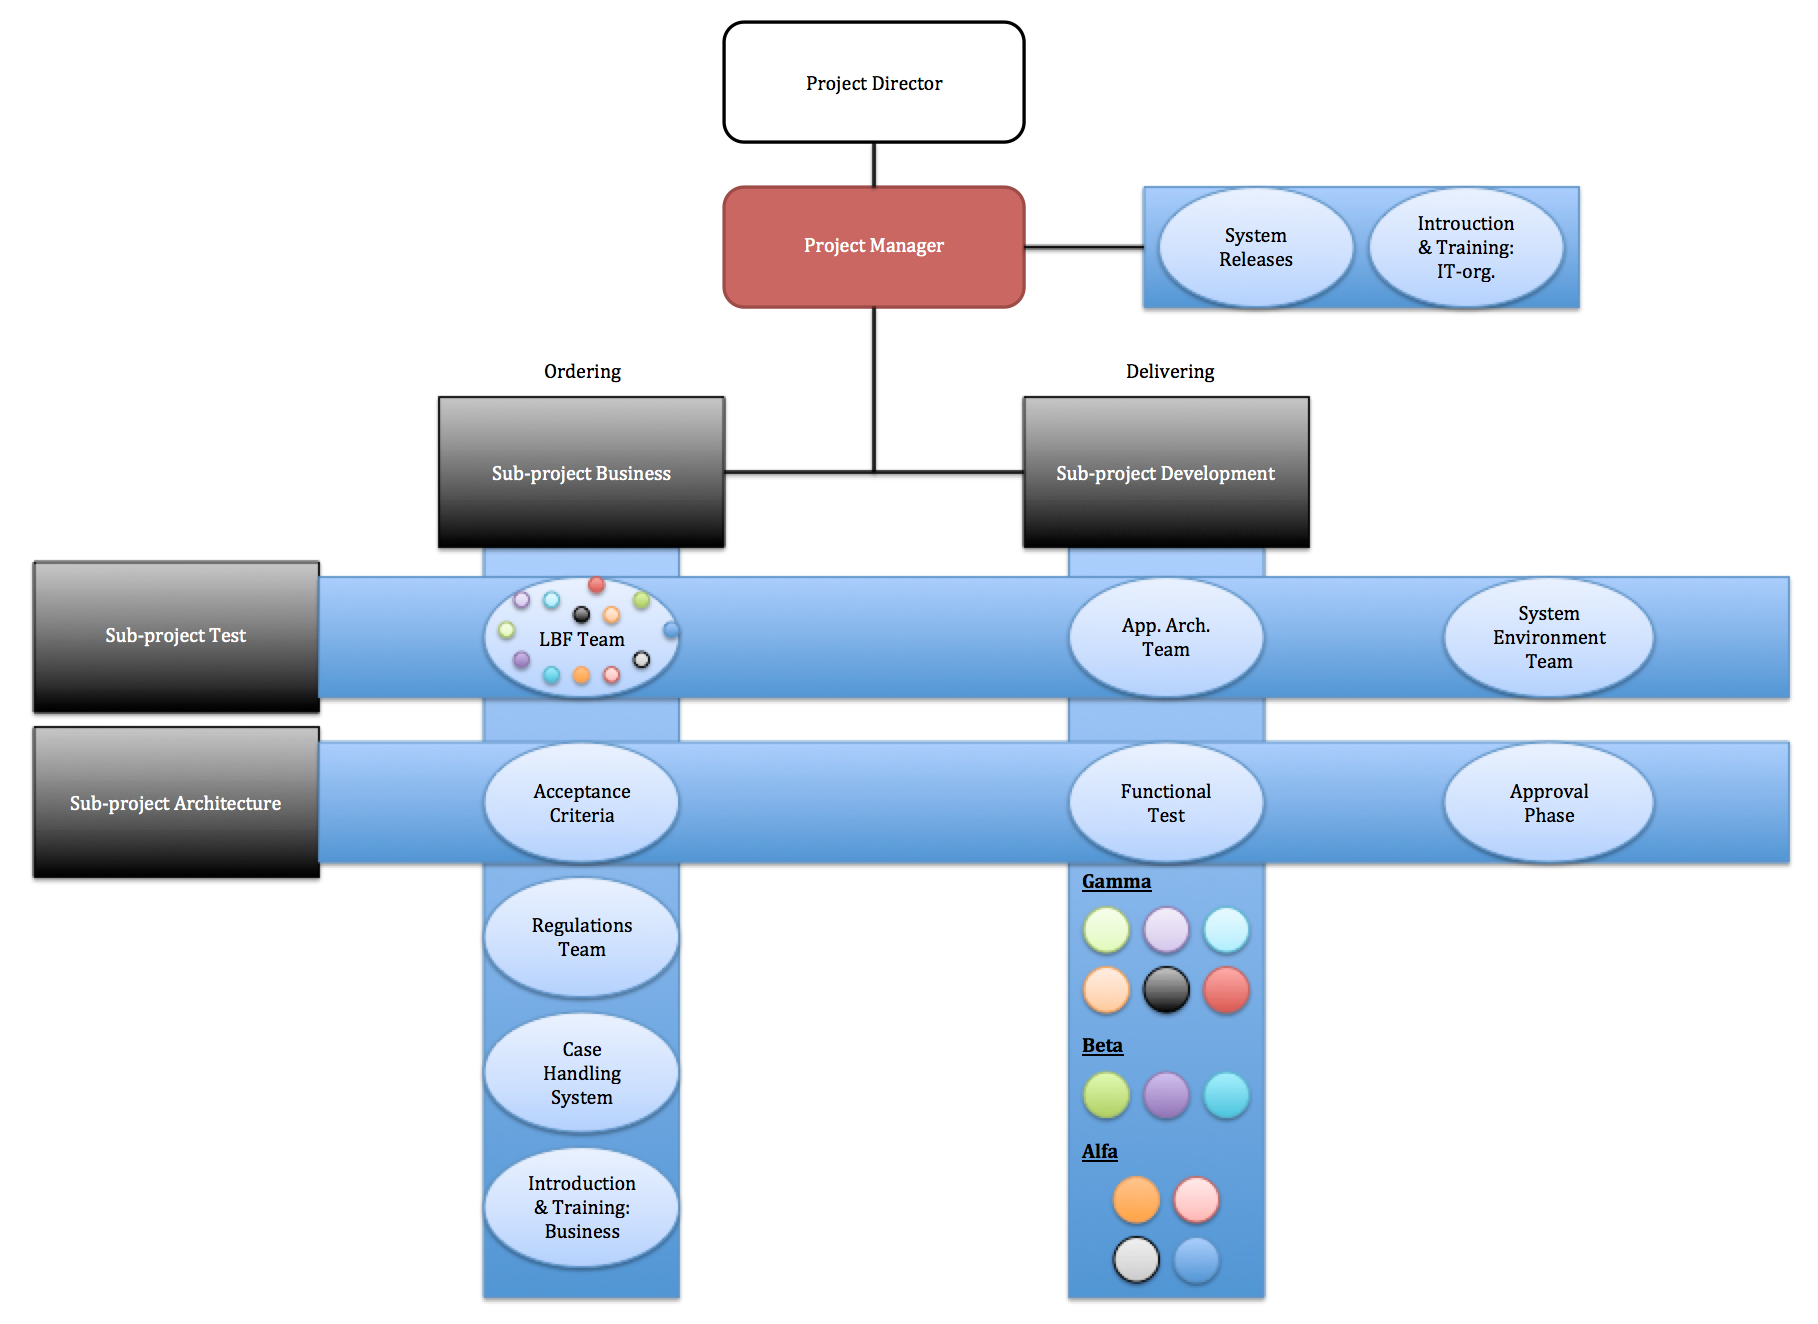
\includegraphics[trim = 40mm 0mm 7mm 0mm,width=180mm]{images/omega_organisation.png}
\caption{Omega-project's organisation.}
\label{omega}
\end{figure}

\begin{figure}[H]
\centering
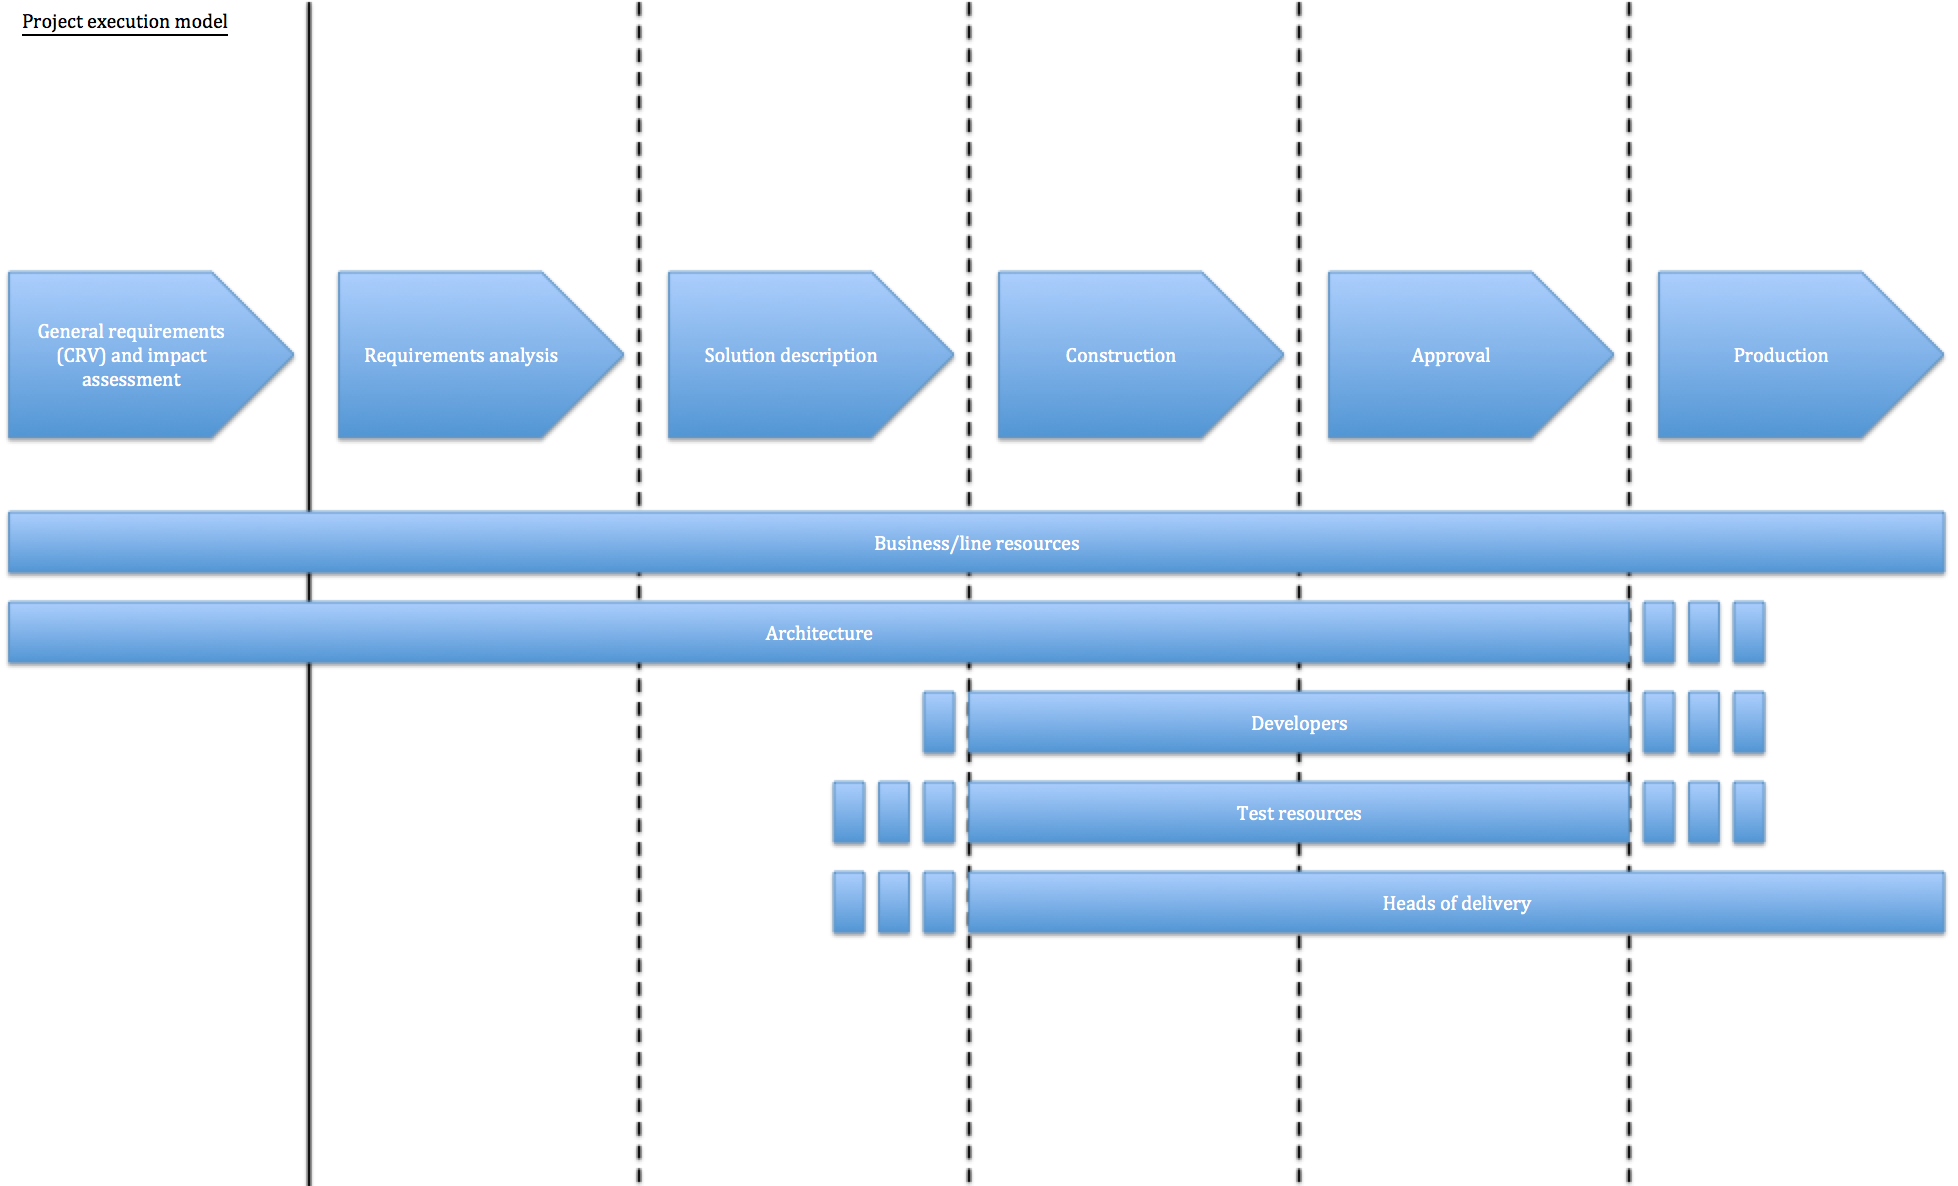
\includegraphics[angle=90, trim = 0mm 0mm 20mm 0mm,width=160mm, height=230mm]{images/execution_model.png}
\caption{Project execution model.}
\label{project_execution}
\end{figure}

\begin{figure}[H]
\centering
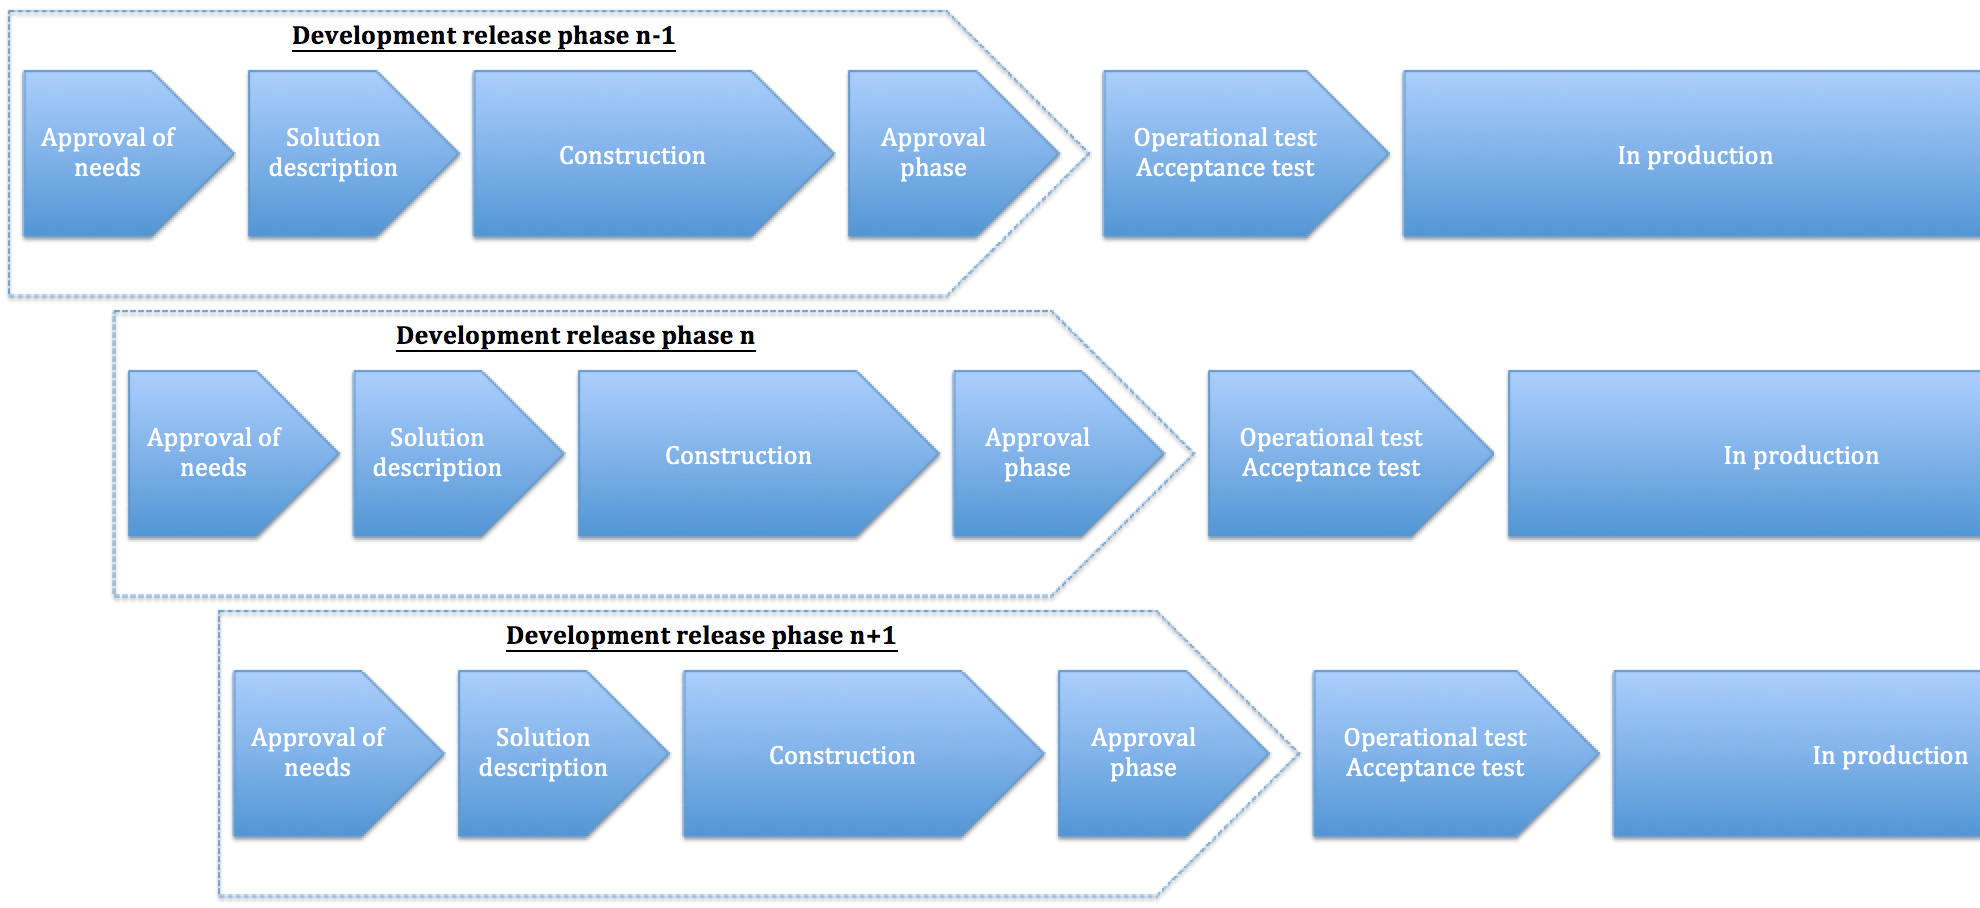
\includegraphics[angle=90, trim = 0mm 0mm 20mm 0mm,width=160mm, height=230mm]{images/initial_development_process}
\caption{Initial development process.}
\label{initial_development_process}
\end{figure}

\begin{table}[H]
\begin{center}
    \begin{tabular}{| p{6cm} | p{9cm} |}
    \hline
    \textbf{Coordination mechanism} & \textbf{Description of mechanism} \\ \hline
    Metascrum & \\ \hline
    Planning day & Ulike nivåer (prosjekt, leverandør og team), utviklerforum (leverandørnivå, ikke på tvers av hele prosjektet), Iterasjonsoppstart(?) \\ \hline
    Dependency meeting & \\ \hline
    Solution description / ``Master plan'' & negotiation and estimation meetings part of solution description meetings \\ \hline
    Wiki/Jira/Confluence & \\ \hline
    Jabber & \\ \hline
    Open-space & \\ \hline
    Lunch seminars & \\ \hline
    Demo & \\ \hline
    Front-end meeting & \\ \hline
    Technical architecture forum & \\ \hline
    Architecture board & \\ \hline
    Business & \\ \hline
    Bug-board meetings  & \\ \hline
    \end{tabular}
    \caption{Coordination mechanisms used across the whole Omega-project.}
    \label{cmuatwo}
\end{center}
\end{table}

%Feil å kalle det sub-projects?
\begin{table}[H]
\begin{center}
    \begin{tabular}{| p{6cm} | p{9cm} |}
    \hline
    \textbf{Coordination mechanism} & \textbf{Description of mechanism} \\ \hline
    Scrum-of-Scrums & \\ \hline
    Stand-up & \\ \hline
    Pre-planning day & \\ \hline
    Technical corner & Beta \\ \hline
    Experience forum & Alpha \\ \hline
    Board discussion & \\ \hline
    Retrospective & Different levels at Alpha (team, solution description and project management), Global retrospektiv testet ut på Beta \\ \hline
    Technical architecture meeting & \\ \hline
    Functional architecture meeting & \\ \hline
    Supplier meeting & Alpha \\ \hline
    Meeting about queue & Alpha \\ \hline
    \end{tabular}
    \caption{Coordination mechanisms used across sub-projects in the Omega-project.}
    \label{cmuasito}
\end{center}
\end{table}

\begin{table}[H]
\begin{center}
    \begin{tabular}{| p{6cm} | p{9cm} |}
    \hline
    \textbf{Mechanism/Aspect} & \textbf{Description} \\ \hline
    Co-location & \\ \hline
    Informal communication & \\ \hline
    Trust & \\ \hline
    Joint coffee break & Alpha (generelt?) \\ \hline
    Pair-programming & \\ \hline
    Self-organising & \\ \hline
    Rotation of team members & \\ \hline
    Rotation of team placement & \\ \hline
    Alfa/Beta-personnel placed in Gamma teams & \\ \hline
    Project management in same location & ``Walking around, talking around'' \\ \hline
    Continuous planning & \\ \hline
    3-level hierarchy from product owner & \\ \hline
    \end{tabular}
    \caption{Other coordination mechanisms and important aspects.}
    \label{ocmaia}
\end{center}
\end{table}